\documentclass{article}
\usepackage{amsmath}
\usepackage{graphicx}
\usepackage{fullpage}

\begin{document}
\title{Motivation and Methods}
\author{Shelby Scott}
\date{\today}
\maketitle

\section*{Motivation}
% Crimes over time in Chicago
% Crimes by month
\begin{figure} [htbp] \centering
 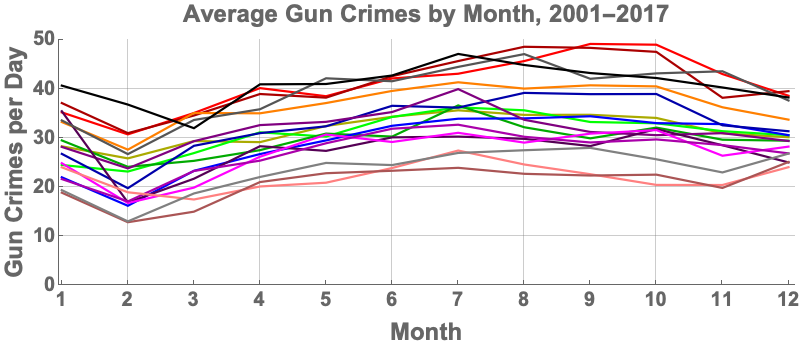
\includegraphics[scale=0.5]{figures/AverageCrimeData.png}
 \caption{The average number of gun crimes by month in Chicago from 2001-2017. Each line represents a different year and there is a pattern evident in which during colder months with more precipitation, there are fewer gun crimes. Meanwhile, in warmer, less wet months, there is less gun crime. Therefore, there are ecological factors that play into levels of gun crime.}
\end{figure}

\begin{figure}[htbp] \centering
 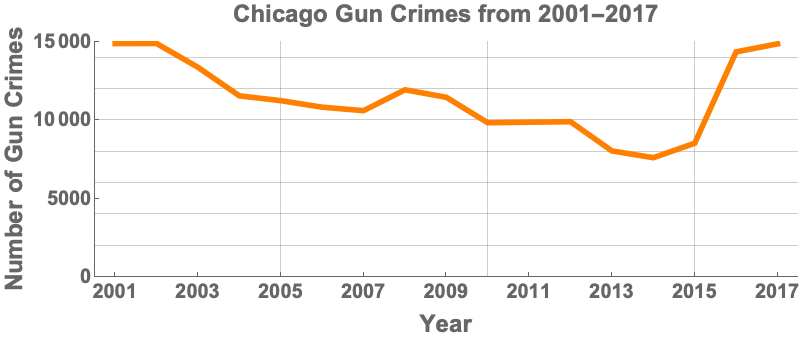
\includegraphics[scale=0.60]{figures/YearlyCrimeData.png}
 \caption{The number of gun crimes in Chicago by year from 2001-2017. There was a fairly regular decline in gun crimes from 2001-2014, before a spike occurred. There is not yet a conclusion about what exactly caused this spike in crimes.}
\end{figure}

\pagebreak
\section*{Methods}
% CA representations
% Histogram of crime
\begin{figure} [htbp] \centering
 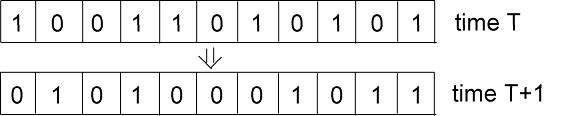
\includegraphics[scale=0.70]{figures/SimpleCA_2Gen.jpg}
 \caption{A simple two generation cellular automata model that follows the local rules present in the table below. Source: http://eric\_rollins.home.mindspring.com/introProgramming/hw5.html}
\end{figure}

\begin{figure} [htbp] \centering
 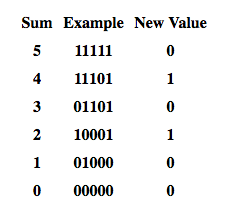
\includegraphics[scale=0.80]{figures/SimpleCA_TransTable}
 \caption{The transition table for the two generation cellular automata model shown above. In each time step, the cells sum the contributions of the two cells to the left and the two cells to the right, then update their state based on this chart. Source: http://eric\_rollins.home.mindspring.com/introProgramming/hw5.html}
\end{figure}

\begin{figure} [htbp] \centering
 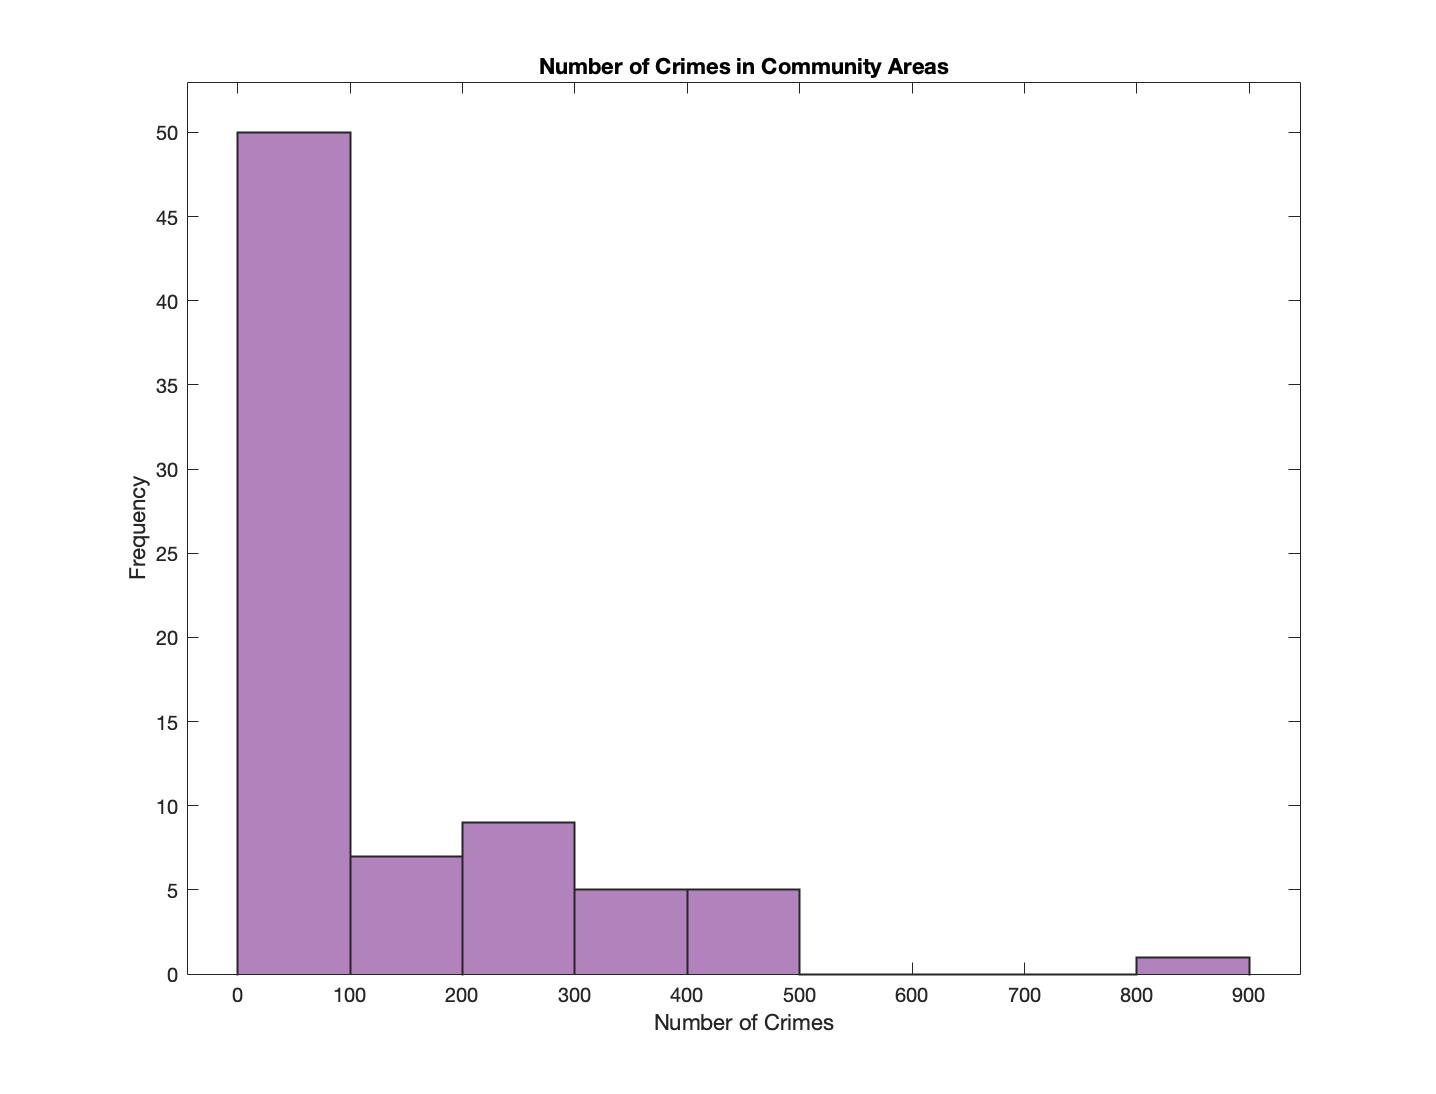
\includegraphics[scale=0.35]{figures/CrimeCountHist.jpg}
 \caption{The histogram of crime counts in Chicago for 2008. The distribution is non-normal and therefore the statistical tests used must take this into account. Because the variance of this data is far larger than the mean ($\mu = 128.88$, $\sigma = 2.29 \times 10^4$), we need to use a negative binomial distribution instead of a Poisson distribution.}
\end{figure}

\end{document}